\section{Bridges in HECRAS and \anuga{} using an internal boundary operator}
This test compares a prismatic channel flow with a bridge in HECRAS and ANUGA.
A 10m wide, 1000m long channel (slope of 1/200, bankfull depth of 1m,
rectangular cross-section) flows through a floodplain (10m wide on either side
of the channel) (Figure~\ref{schematic}). 500m downstream there is a bridge
with a 1.3m high rectangular opening over the channel, and a deck elevation of
-1m. In HECRAS the bridge is modelled using the energy method, see the
associated HECRAS files for details. In ANUGA the bridge is modelled by
inserting the bridge deck (upper chord) into the topography, with an internal
boundary operator to describe the bridge underflow. The rating curves for the
bridge underflow (used to compute the bridge discharge from the upstream and
downstream stage) were derived for ANUGA from HECRAS by raising the upper chord
of the bridge in HECRAS (far about the flow) and computing internal boundary
tables, which were then copied into a csv file for use by ANUGA. The bridge
overflow in ANUGA is modelled with the shallow water equations (although
riverwalls could also be used to apply weir type equations instead). Both
models have a uniform Manning's n of 0.045, which prevents too much
supercritical flow in HECRAS (and the associated numerical supression of the
inertial terms that HECRAS uses to retain stability).

\begin{figure}
\begin{center}
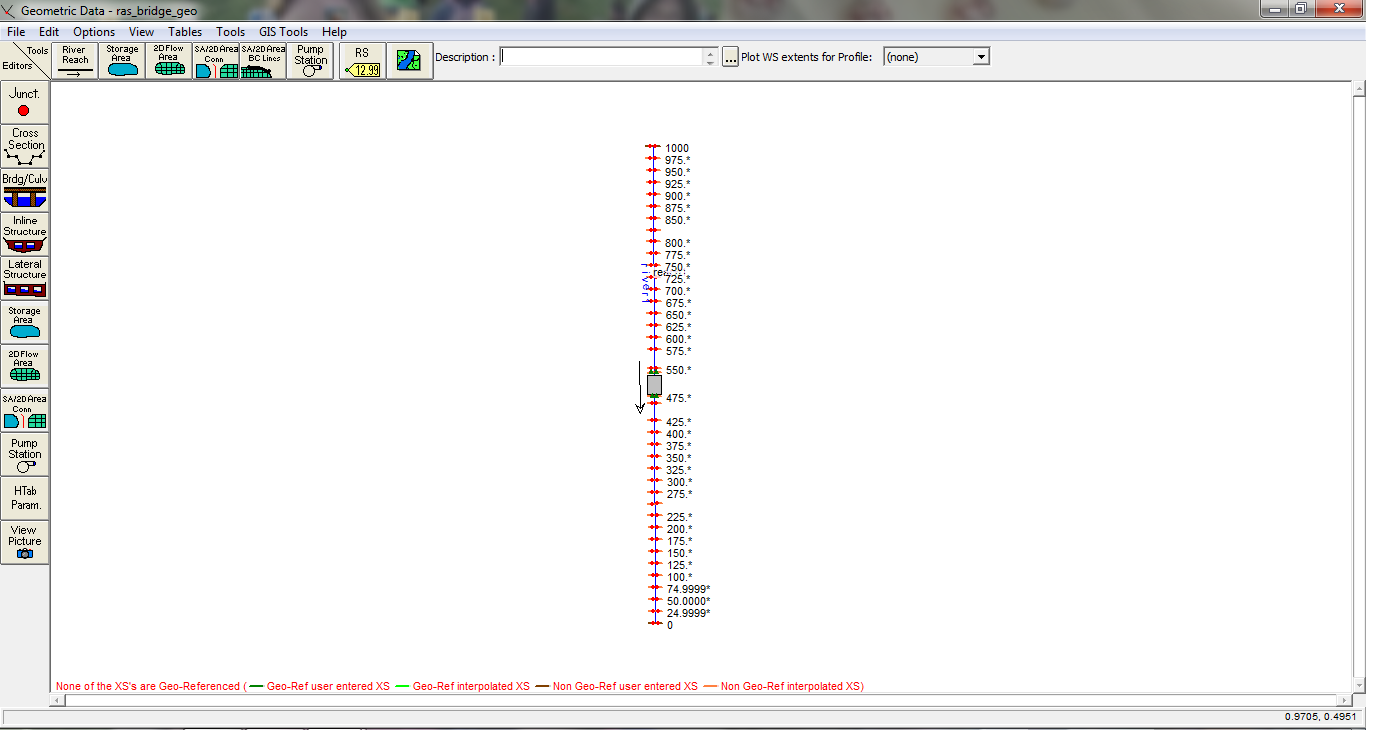
\includegraphics[width=1.0\textwidth]{hecras_bridge_test/RASGeometry_Bridge.png}
\end{center}
\caption{Screenshot showing the HECRAS model geometry schematization}
\label{schematic}
\end{figure}


A discharge timeseries is imposed upstream for both models, with the discharge
increasing from 1m$^3$/s initially to 70m$^3$/s at the end of the simulation.
Details of the model setup can be seen in the code / input files in this
directory.

\subsection{Results}

Figure~\ref{Reach} show stage timeseries at various stations downstream in each
model. The ANUGA and HECRAS results are qualitatively similar, but differ in
detail. 

\begin{figure}
\begin{center}
\includegraphics[width=0.9\textwidth]{CENTRAL_CHANNEL.png}
\end{center}
\caption{Stage at various points downstream in the channel}
\label{Reach}
\end{figure}

In early stages of the simulation when discharges are lower, ANUGA shows stages
slightly below HECRAS (particularly away from the bridge). This reflects the
fact that HECRAS models side-wall friction while ANUGA does not, so there is
more drag in the HECRAS model. 

As the discharge increases, the models show more deviation around the bridge
and upstream, and ultimately approach different steady states. At high flows,
the main reason for this is that they use different methods to model the bridge
overflow, which begins when station 525 exceeds -1m. ANUGA uses the shallow
water equations, while HECRAS uses an energy method. Even before this, the
models show differences once the flow goes overbank (above -2.4m at station
525). Because the ANUGA model here has a fairly coarse mesh, numerical
diffusion causes additional drag for overbank flows. 

Several additional factors will contribute to deviations between the models. ANUGA
models cross-channel variations in the water surface elevation, which is
assumed constant in HECRAS. The under-bridge flux in ANUGA is based on the
water elevations in the central channel up-and-down stream of the bridge, thus
the 2D representation will have an effect on the under-bridge flow. The models
also flux the momentum under the bridge in different ways. ANUGA's method is to
compute the average momentum in each direction along the upstream bridge
inflow, and assume that this is advected by the discharge (as computed from the
internal boundary rating curves). HECRAS's method is based on the energy
equation. 


